\newpage
\section {Билет 13. Обработка текстов. Морфологический анализ, tf*idf, ранжирование, исправление опечаток, классификация, кластеризация, поиск дубликатов.}

Пусть у нас есть пачка текстов, которую мы будем исследовать \\
Методы представления текстов
\begin{itemize}
\item множетсвенный. Текст представляется как множество слов, для которых не определено отношение порядка. Преимущество - простота. Для вычисления сходства двух текстов используется простая формула $k = \frac {|A \cup B|}{|A \cap B|}$. Если коэффициент большой, то тексты похожи друг на друга.
\item векторная модель. Пусть есть выделенные  "базисные" слова $w_1, w_2, \dots w_n$, тогда текст представляется вектором в n-мерном пространстве, где координаты вектора строятся так: i - ая координата это количество вхождения слова $w_i$ в текст. Но на практике используют другой способ определения координат (о нем ниже)  
\item линейная модель.
\item семантическая (очень сложная и мы ее особо не обсуждали).
\end{itemize}

Модель tf*idf\\
\url {https://ru.wikipedia.org/wiki/Векторная_модель}
tf для слова $w_i$ в тексте $T_j$ определяется так: 
 $tf = log (Q)$, Q - сколько раз $w_i$ встретилось в $T_j$.  \\
idf для слова $w_i$ в тексте $T_j$ определяется так: 
$idf = \frac{1}{log(P)}$, P - количество документов, в которых встречается слово $w_i$ \\
На практике используют именно произведение $tf*idf$ - означающее важность слова в документе. Отражает закон Зипфа:
На графике по вертикальной оси откладывается важность (т.е. tf*idf) по горизонтальной частота встречаемости слова в конкретном документе.
Выделяется три зоны: \\
1 - редкие слова, слова придуманные автором или опечатки \\
2 - ключевые слова, определяющие текст \\
3 - обычные слова связки \\

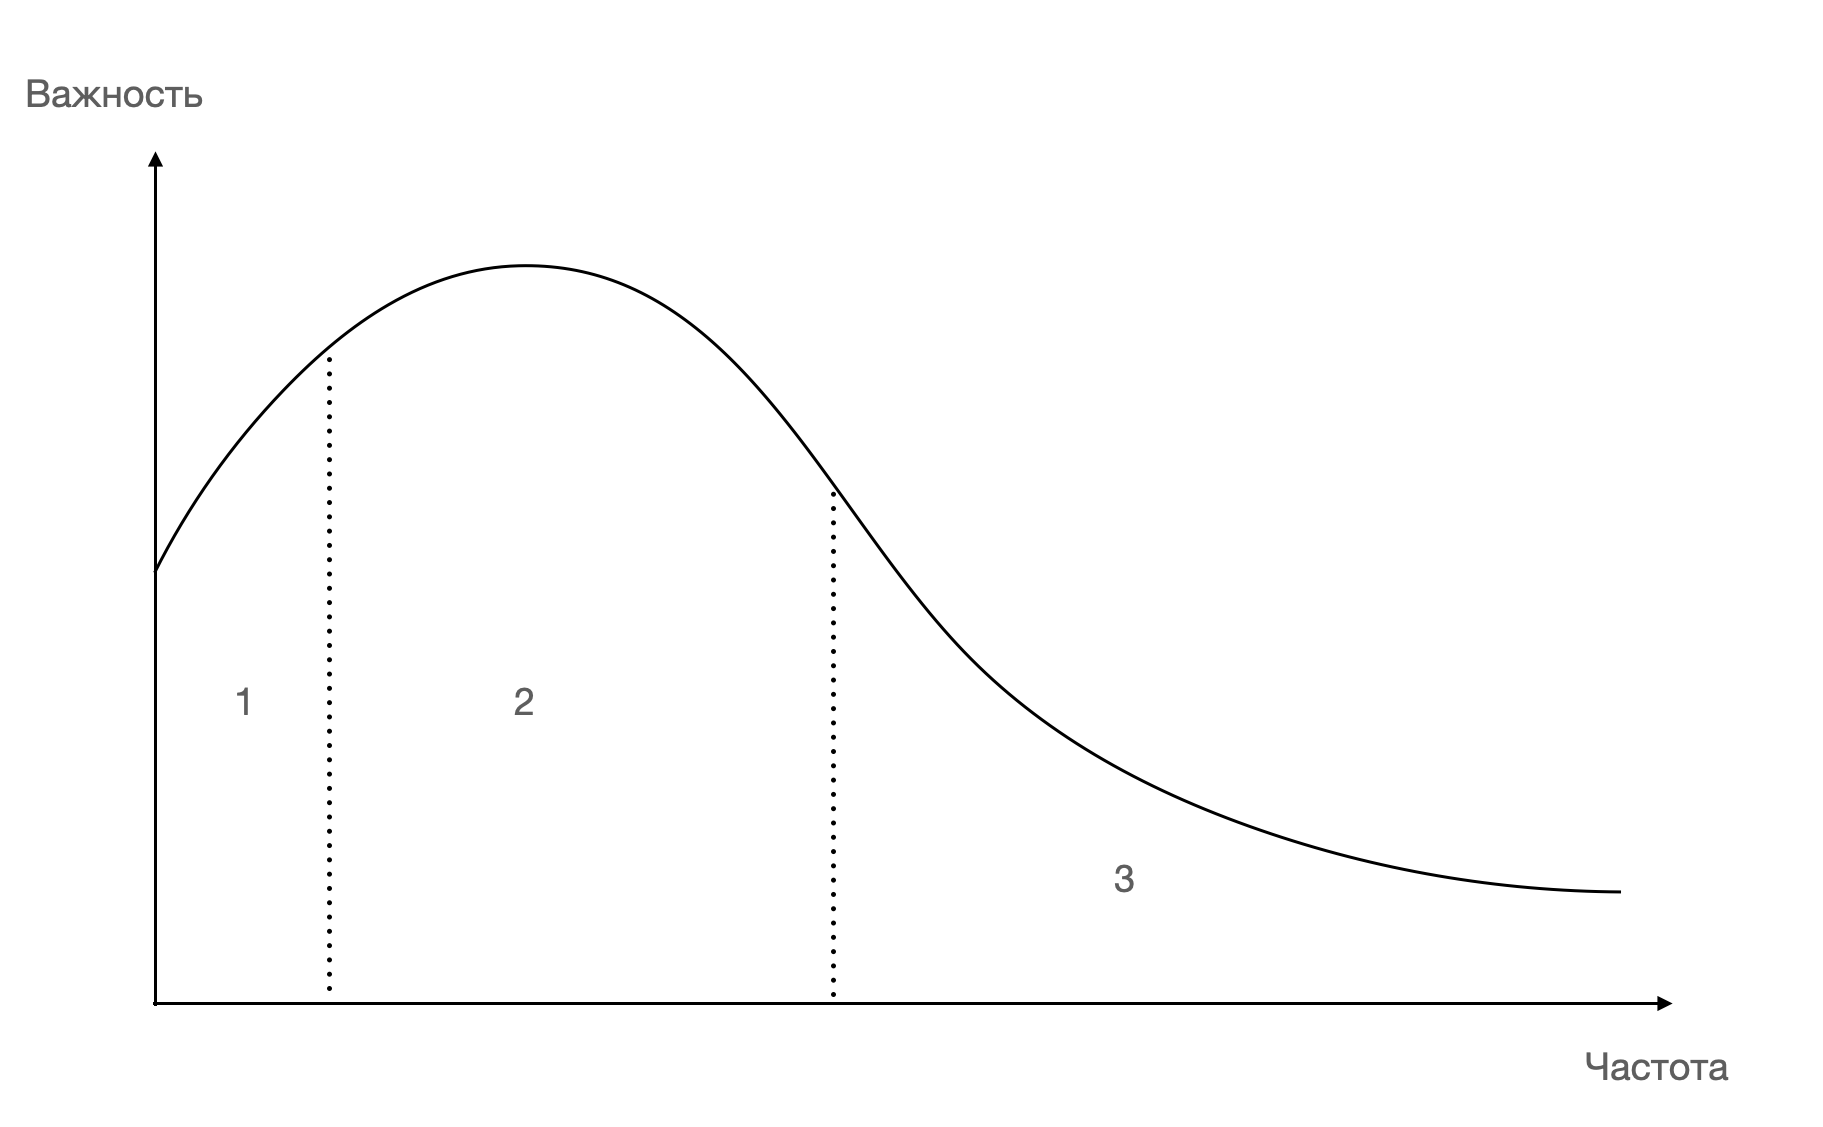
\includegraphics[width=0.5\linewidth]{13/Zipf}

Мера близости текстов A и B в векторной модели - косинус угла между векторами A и B.

\subsubsection {Посторение векторов}
Перед построением векторов сначала несколько унифицируют используемые слова, для этого используют морфологический анализ.
Морфологический анализ может быть словарным (со словарем основ и окончаний или словарем словоформ) или бессловарным (только со словарем окончаний; словарь окончаний может быть встроен в алгоритм морфологического анализа). Бессловарный метод используется только для определения переменной морфологической информации (не всегда однозначно), а словарный — во всех остальных случаях. 

\subsubsection {Исправление опечаток}
Расстояние по Левинштейну:
Элементарная операция по Левинштейну - это добавление буквы, удаление буквы или замена одной буквы на другую. Расстояние это количество операций необходимое для того, чтобы из одного слова получить другое. Например, слова aabb, aabbb, aab, aacb находятся на одинаковом расстоянии (расстояние равно 1). Далее, чтобы исправить опечатку необходимо найти ближайшее слово по Левинштейну. 
Возникает следующая проблема: как быстро найти ближайшее слово ? \\
На практике используют обход по дереву. + вероятность замены одной буквы на другую, например, о-а - большая вероятность, а з-ф - маленькая

\subsubsection {Поиск дубликатов}
Если необходимо решить задачу на полное совпадение текстов, то она делается очень просто. Для каждого документа берется хэш функция. С большой вероятностью документы с совпадающем хэшем - совпадают. Но на практике необходимо искать не в точности совпадающие тексты, а просто похожие. В таком случае используют понятие N-грамм.  \\
Определение: N-грамма — последовательность из n элементов. Например для текста: Мама мыла раму, все 4 граммы имеют вид: мама, амам, мамы, амыл, мыла, ылар, лара, арам, раму.  \\
Теорема. Если документы почти совпадают, то и тексты почти совпадают. \\
Это отличный способ, сравнивать все N-граммы, но есть одна проблема - их очень много и сравнение всех N-грамм двух текстов займет много времени. Поэтому действуют следующим образом

\begin {itemize}
\item Берутся все N-граммы двух текстов и к ним применяется какой-нибудь хеш. (хэш функция от N - граммы называется называется шинглом)
\item Береться 84 шингла (значения хэш функции), они объединяются в 12 групп
\item На каждой группе шинглов опять вычисляется хэш функция. (начение хэш функции на группе шинглов называется супершинглом)
\item Если у двух текстов совпадает хотя бы один супершингл,  то они потенциально совпадают.
\end {itemize}

\subsubsection {Классификация}
Классификация - разделение на текстов группы, которые мы заранее определили.


